\documentclass[10pt]{extarticle}

\usepackage[margin=1.8cm]{geometry}
\usepackage{amsmath,amssymb}
\usepackage{booktabs}
\usepackage{enumitem}
\usepackage{graphicx}
\usepackage{xcolor}
\usepackage[
  colorlinks=true,
  linkcolor=blue!50!black,
  urlcolor=blue!60!black
]{hyperref}

\setlist{itemsep=2pt,topsep=4pt}

\title{Tanaka Certificates: Weekly Research Report}
\author{Filip Morawiec}
\date{20 July 2026}

\begin{document}

\maketitle

\begin{abstract}
This report presents a Residual Deep ICNN certificate whose local-time sign is
safe by construction.  For the enlarged-target Ornstein--Uhlenbeck problem, a
fixed-feature instance was fitted by linear programming and formally verified
on 1,177 cells.  A much larger model can be trained with Adam, but exact cell
discovery does not scale to that model.  Interval bound propagation is
therefore the next verification direction.  Committor functions do not
directly meet the strict certificate conditions, but their transition geometry
may help choose training samples.
\end{abstract}

\tableofcontents

\section{Certificate architecture}

Let $X_t$ satisfy
\begin{equation}
  dX_t=f(X_t)\,dt+\sigma(X_t)\,dW_t.
\end{equation}
The certificate $V$ must be small on the initial set and at least $\beta$ on
the unsafe set and the domain boundary.  Before the process reaches the target
or the level set $\{V\geq\beta\}$, it must also satisfy
\begin{equation}
  V\geq0,
  \qquad
  \mathcal LV\leq-\epsilon.
\end{equation}
If $V$ is piecewise smooth, the multidimensional It\^o--Tanaka formula adds a
local-time term at every interface.  The jump in the normal derivative must
have the correct sign; checking arbitrary interfaces one by one is expensive.

The Residual Deep ICNN avoids that check by writing
\begin{equation}
  \boxed{V(x)=\gamma\bigl(S(x)-C(x)\bigr)},
  \qquad \gamma>0.
\end{equation}
The smooth branch is
\begin{equation}
  S(x)=c+p^\top x+\frac12x^\top Hx
  +\frac12\sum_{k=1}^{m}v_k
  \operatorname{ReLU}(a_k^\top x+b_k)^2.
\end{equation}
Squared ReLU is continuously differentiable, so $S$ is $C^1$ and piecewise
quadratic.  It has no surface-local-time contribution, but its cellwise
Hessian may have either sign.  This ordinary curvature is useful because the
diffusion part of $\mathcal L V$ depends on second derivatives.

The second branch $C$ is a fully input-convex ReLU network.  With
\begin{align}
  z_1(x)&=\operatorname{ReLU}(A_1x+b_1),\\
  z_{\ell}(x)&=\operatorname{ReLU}
  \bigl(A_{\ell}x+W_{\ell}z_{\ell-1}(x)+b_{\ell}\bigr),
  \qquad W_{\ell}\geq0,
\end{align}
its output is $C(x)=a^\top x+b+w^\top z_L(x)$ with $w\geq0$.  The direct
input weights $A_\ell$ are unrestricted, while the hidden-to-hidden and output
weights are made nonnegative using a softplus parameterization.  Since ReLU is
convex and nondecreasing, these constraints make $C$ convex by induction over
the layers.  It is also continuous and piecewise affine.

Consequently, $S$ contributes no singular curvature and the kink curvature of
$C$ is positive semidefinite.  The singular curvature of $V$ is therefore
\begin{equation}
  D^2_{\mathrm{sing}}V=-\gamma D^2_{\mathrm{sing}}C\preceq0.
\end{equation}
This gives the safe local-time sign at every ICNN activation interface without
enumerating adjacent facets.  It does \emph{not} prove the value or ordinary
generator inequalities; those still require formal verification.

If $V\leq\alpha$ on the initial set, these conditions give the reach--avoid
bound
\begin{equation}
  \mathbb P_x(\text{unsafe set or domain exit before target})
  \leq \frac{\alpha}{\beta}.
\end{equation}

\section{Certificate verified with linear programming}

The new verified result uses the harder enlarged-target benchmark
\begin{equation}
  dX_t=-X_t\,dt+0.5\,dW_t
\end{equation}
on $[-1,1.25]\times[-1.25,0.75]$.  The target is $[-0.5,0.5]^2$,
$\beta=2$, and $\epsilon=0.1$.  The initial and unsafe sets are the two small
rectangles shown in Figure~\ref{fig:verified-lp}.

A numerical Poisson solution first provides the desired global shape.  The
ridge locations are then fixed, which makes the unknown piecewise-quadratic
coefficients linear.  A linear program fits these coefficients to the teacher
while enforcing the certificate inequalities.  Finally, the exact verifier
checks every resulting cell; the sampled diagnostics in the plot are only for
visualization.

The verifier returned \emph{verified} with 1,177 cells and no unresolved cells.
It proved the thresholds $\alpha=1.97$, $\beta=2$, and $\epsilon=0.1$, hence
the current probability bound is $\alpha/\beta=0.985$.  This bound is weak, but
the experiment establishes that the architecture, LP fit, and exact verifier
work together on the enlarged-target problem.

\begin{figure}[htbp]
  \centering
  \includegraphics[width=0.94\textwidth]{../../../../second-workspace/tanaka-certificates/output/04604e2_2026-07-16_13-30-33_verified_icnn_poisson_teacher/verified_diagnostics.png}
  \caption{LP-fitted and formally verified certificate.  The panels show the
  Poisson teacher, the certificate, their difference, and $\mathcal LV$.
  The white contour is $V=\beta$; the exact result is based on all 1,177 cells,
  not on the plotted grid.}
  \label{fig:verified-lp}
\end{figure}

\section{Training and verification at larger scale}

Linear programming is possible here because the feature geometry is fixed.
It is not a practical long-term training method for a deep model whose features
must also be learned.  The Adam experiment in Figure~\ref{fig:large-icnn} used
16 smooth hinges and a four-layer width-79 ICNN, for 19,824 trainable
parameters.  It learned a useful surface, but it did not simultaneously satisfy
the initial, unsafe, boundary, and generator conditions.  Sampling and
counterexample replay improve the fit, yet optimization can move a violation
from one condition to another.

For comparison, Figure~\ref{fig:plain-relu} shows a depth-4, width-80 plain
ReLU network with 19,761 parameters.  It passed the same dense empirical audit.
The signed margins of the two runs are:

\begin{center}
\begin{tabular}{lrr}
\toprule
Condition & Residual Deep ICNN & Plain ReLU\\
\midrule
Initial & $-0.2704$ & $+0.0146$\\
Unsafe & $-0.4188$ & $+2.5601$\\
Domain boundary & $-0.4038$ & $+0.0131$\\
Nonnegative & $+0.0669$ & $+0.0070$\\
Generator & $-0.3879$ & $+0.0109$\\
\bottomrule
\end{tabular}
\end{center}

This comparison is a negative control, not evidence that plain ReLU is the
better certificate.  A ReLU network is affine inside each activation cell, so
its classical Hessian is zero there and the sampled generator omits diffusion
curvature.  Its gradient jumps at cell boundaries with no controlled sign,
which creates unverified local-time terms.  The Residual Deep ICNN has the
correct interface sign by construction; the plain ReLU does not.

\begin{figure}[htbp]
  \centering
  \includegraphics[width=0.92\textwidth]{../../../output/c046bb0_2026-07-20_11-38-08_adam_certificate_experiment/training_diagnostics.png}
  \caption{Adam-trained 19,824-parameter Residual Deep ICNN.  The local-time
  sign is structurally safe, but the dense audit still finds value and
  generator violations.  Exact verification was not run because cell
  discovery is intractable at this size.}
  \label{fig:large-icnn}
\end{figure}

\begin{figure}[htbp]
  \centering
  \includegraphics[width=0.92\textwidth]{../../../output/c046bb0_2026-07-19_19-56-10_plain_relu_certificate/training_diagnostics.png}
  \caption{Empirically feasible 19,761-parameter plain ReLU network.  Its
  pointwise plots do not include activation-interface local time, so this is
  not a valid stochastic certificate despite passing the dense audit.}
  \label{fig:plain-relu}
\end{figure}

The immediate verification bottleneck is cell discovery.  For 16 smooth
ridges followed by four width-79 ReLU layers, a crude region bound is
\begin{equation}
  137\left(1+79+\binom{79}{2}\right)^4
  \approx 1.4\times10^{16}.
\end{equation}
Enumerating activation patterns is therefore infeasible; the present estimate
is about $2\cdot10^{15}$ years.

The next approach is interval bound propagation (IBP) with adaptive splitting.
For a box $B$, verification only needs to prove
\begin{equation}
  \underline V(B)>\beta
  \qquad\text{or}\qquad
  \overline{\mathcal LV}(B)\leq-\epsilon.
\end{equation}
Ambiguous boxes are split until one inequality holds.  ReLU bounds are simple
and cheap, whereas smooth activations generally need more expensive nonlinear
relaxations.  The local-time sign remains guaranteed by the architecture and
does not enter this branch-and-bound search.

\section{Committor functions as a sampling guide}

For two disjoint sets $A$ and $B$, the committor is
\begin{equation}
  q(x)=\mathbb P_x(\tau_B<\tau_A).
\end{equation}
In this project, let $A$ be the target and let $B$ be failure: the unsafe set or
domain exit.  Then $q(x)$ is simply the probability of failure before success
from state $x$.  It equals $0$ on the target, $1$ on the failure boundary, and
satisfies $\mathcal Lq=0$ between them.  Values near $q=1/2$ identify states for
which both outcomes are plausible, so these states contain more useful
transition information than points deep inside either region.

For reversible overdamped Langevin dynamics, write the inverse temperature as
$\kappa$ to distinguish it from the certificate threshold $\beta$:
\begin{equation}
  dX_t=-\nabla U(X_t)\,dt+\sqrt{2\kappa^{-1}}\,dW_t,
  \qquad
  \mathcal L=-\nabla U\cdot\nabla+\kappa^{-1}\Delta.
\end{equation}
Let $D=\Omega\setminus(A\cup B)$.  The committor is equivalently the minimizer
of the weighted Dirichlet energy
\begin{equation}
  q=\underset{u\in H^1(D)}{\operatorname{argmin}}
  \underbrace{\int_D\lVert\nabla u(x)\rVert^2
  e^{-\kappa U(x)}\,dx}_{\mathcal E(u)},
  \qquad
  u|_{\partial A}=0,\quad u|_{\partial B}=1,
  \label{eq:committor-variational}
\end{equation}
with the appropriate condition on the outer boundary of $\Omega$.  This
optimization has a probabilistic interpretation: among functions separating
$A$ and $B$, the committor has minimum energy under the equilibrium weight
$e^{-\kappa U}$.

The connection to the backward equation follows from the first variation.  For
any perturbation $\eta$ that is zero on $\partial A\cup\partial B$,
\begin{align}
  0
  &=\left.\frac{d}{ds}\mathcal E(q+s\eta)\right|_{s=0}\\
  &=2\int_D \nabla q\cdot\nabla\eta\,e^{-\kappa U}\,dx
   =-2\int_D\eta\,\nabla\!\cdot
   \left(e^{-\kappa U}\nabla q\right)dx.
\end{align}
Hence $\nabla\!\cdot(e^{-\kappa U}\nabla q)=0$, which is equivalent to
$\mathcal Lq=0$.  This also shows why the variational loss is attractive for
neural networks: it needs only first derivatives of $q$, whereas a direct PDE
residual $\lVert\mathcal Lq\rVert^2$ needs second derivatives.

With a neural approximation $q_\theta$ and interior sampling density $r$, a
Monte Carlo training objective has the form
\begin{align}
  J(\theta)
  ={}&\mathbb E_{X\sim r}
  \left[\frac{\lVert\nabla q_\theta(X)\rVert^2
  e^{-\kappa U(X)}}{r(X)}\right] \\
  &+\lambda_A\mathbb E_{X\sim\partial A}[q_\theta(X)^2]
  +\lambda_B\mathbb E_{X\sim\partial B}[(q_\theta(X)-1)^2].
  \label{eq:committor-neural-loss}
\end{align}
The last two terms enforce the boundary values.  The interior integrand
$\lVert\nabla q_\theta\rVert^2e^{-\kappa U}$ is also an error indicator: it is
large where the current model places transition energy.  DASTR therefore fits
a generative model to the normalized density
\begin{equation}
  p_{U,q_\theta}(x)\propto
  \lVert\nabla q_\theta(x)\rVert^2e^{-\kappa U(x)}
\end{equation}
and uses its samples in the next optimization round.  This exact variational
form relies on reversible Langevin dynamics; a general non-reversible SDE
requires a different weak formulation or a residual loss.

Figure~\ref{fig:khoo-committor} gives a concrete example.  The stochastic
dynamics spend most of their time near the metastable sets $A$ and $B$, while
the committor changes between $0$ and $1$ across the region separating them.
The neural approximation reproduces this global transition geometry.  The
important difficulty is visible in the first panel: ordinary trajectory data
are concentrated near $A$ and $B$, not where the committor changes most.

\begin{figure}[htbp]
  \centering
  \begin{minipage}{0.32\textwidth}
    \centering
    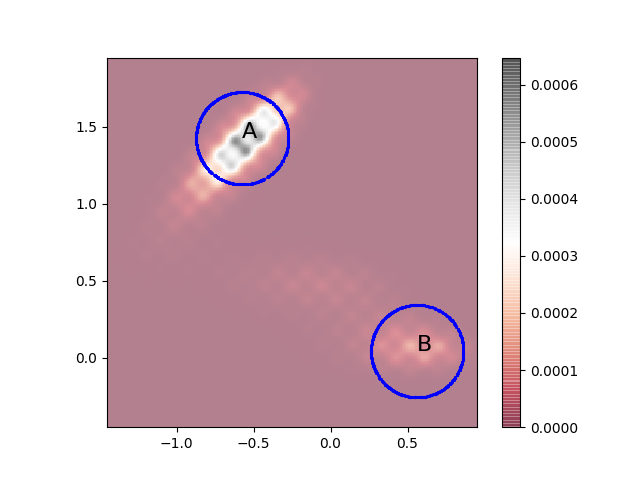
\includegraphics[width=\linewidth]{img/khoo-rugged-mueller-density.png}
    \small (a) Equilibrium density
  \end{minipage}
  \begin{minipage}{0.32\textwidth}
    \centering
    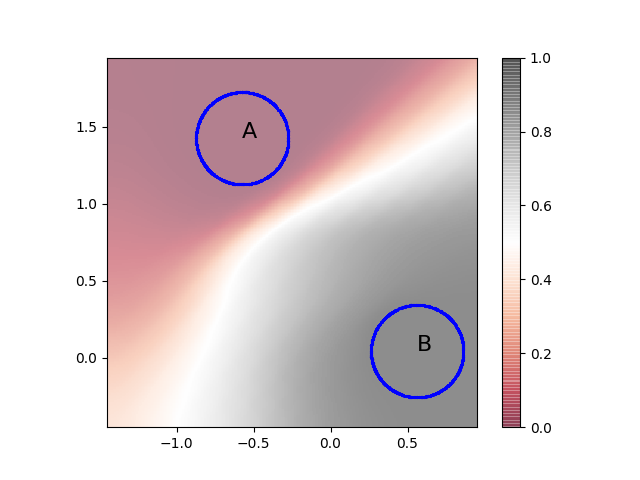
\includegraphics[width=\linewidth]{img/khoo-rugged-mueller-committor.png}
    \small (b) Reference committor
  \end{minipage}
  \begin{minipage}{0.32\textwidth}
    \centering
    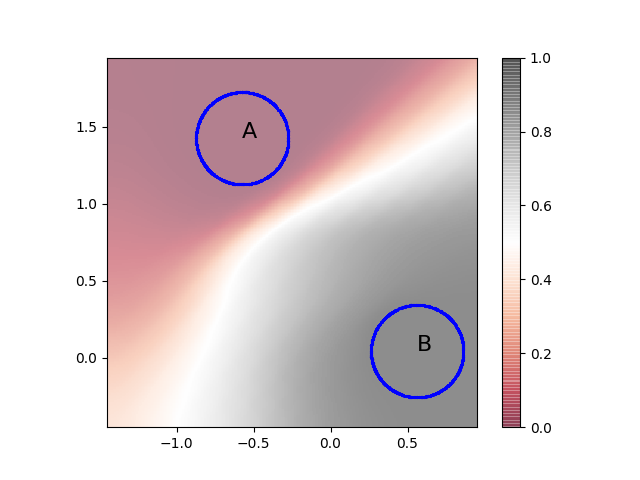
\includegraphics[width=\linewidth]{img/khoo-rugged-mueller-nn.png}
    \small (c) Neural committor
  \end{minipage}
  \caption{Rugged M\"uller example at temperature $T=22$.  The density is
  concentrated in the metastable regions, whereas the committor describes the
  transition from $A$ to $B$.  Reproduced from Figure~6 of
  \href{https://arxiv.org/abs/1802.10275}{Khoo, Lu, and Ying}.}
  \label{fig:khoo-committor}
\end{figure}

DASTR addresses this data problem with the feedback loop in
Figure~\ref{fig:dastr-workflow}.  A provisional committor determines a sampling
density that emphasizes the transition region.  New samples from that density
are used to retrain the committor, and the process is repeated.  This is closely
related to counterexample replay in certificate training: the current model
decides where the next training points should be placed.

\begin{figure}[htbp]
  \centering
  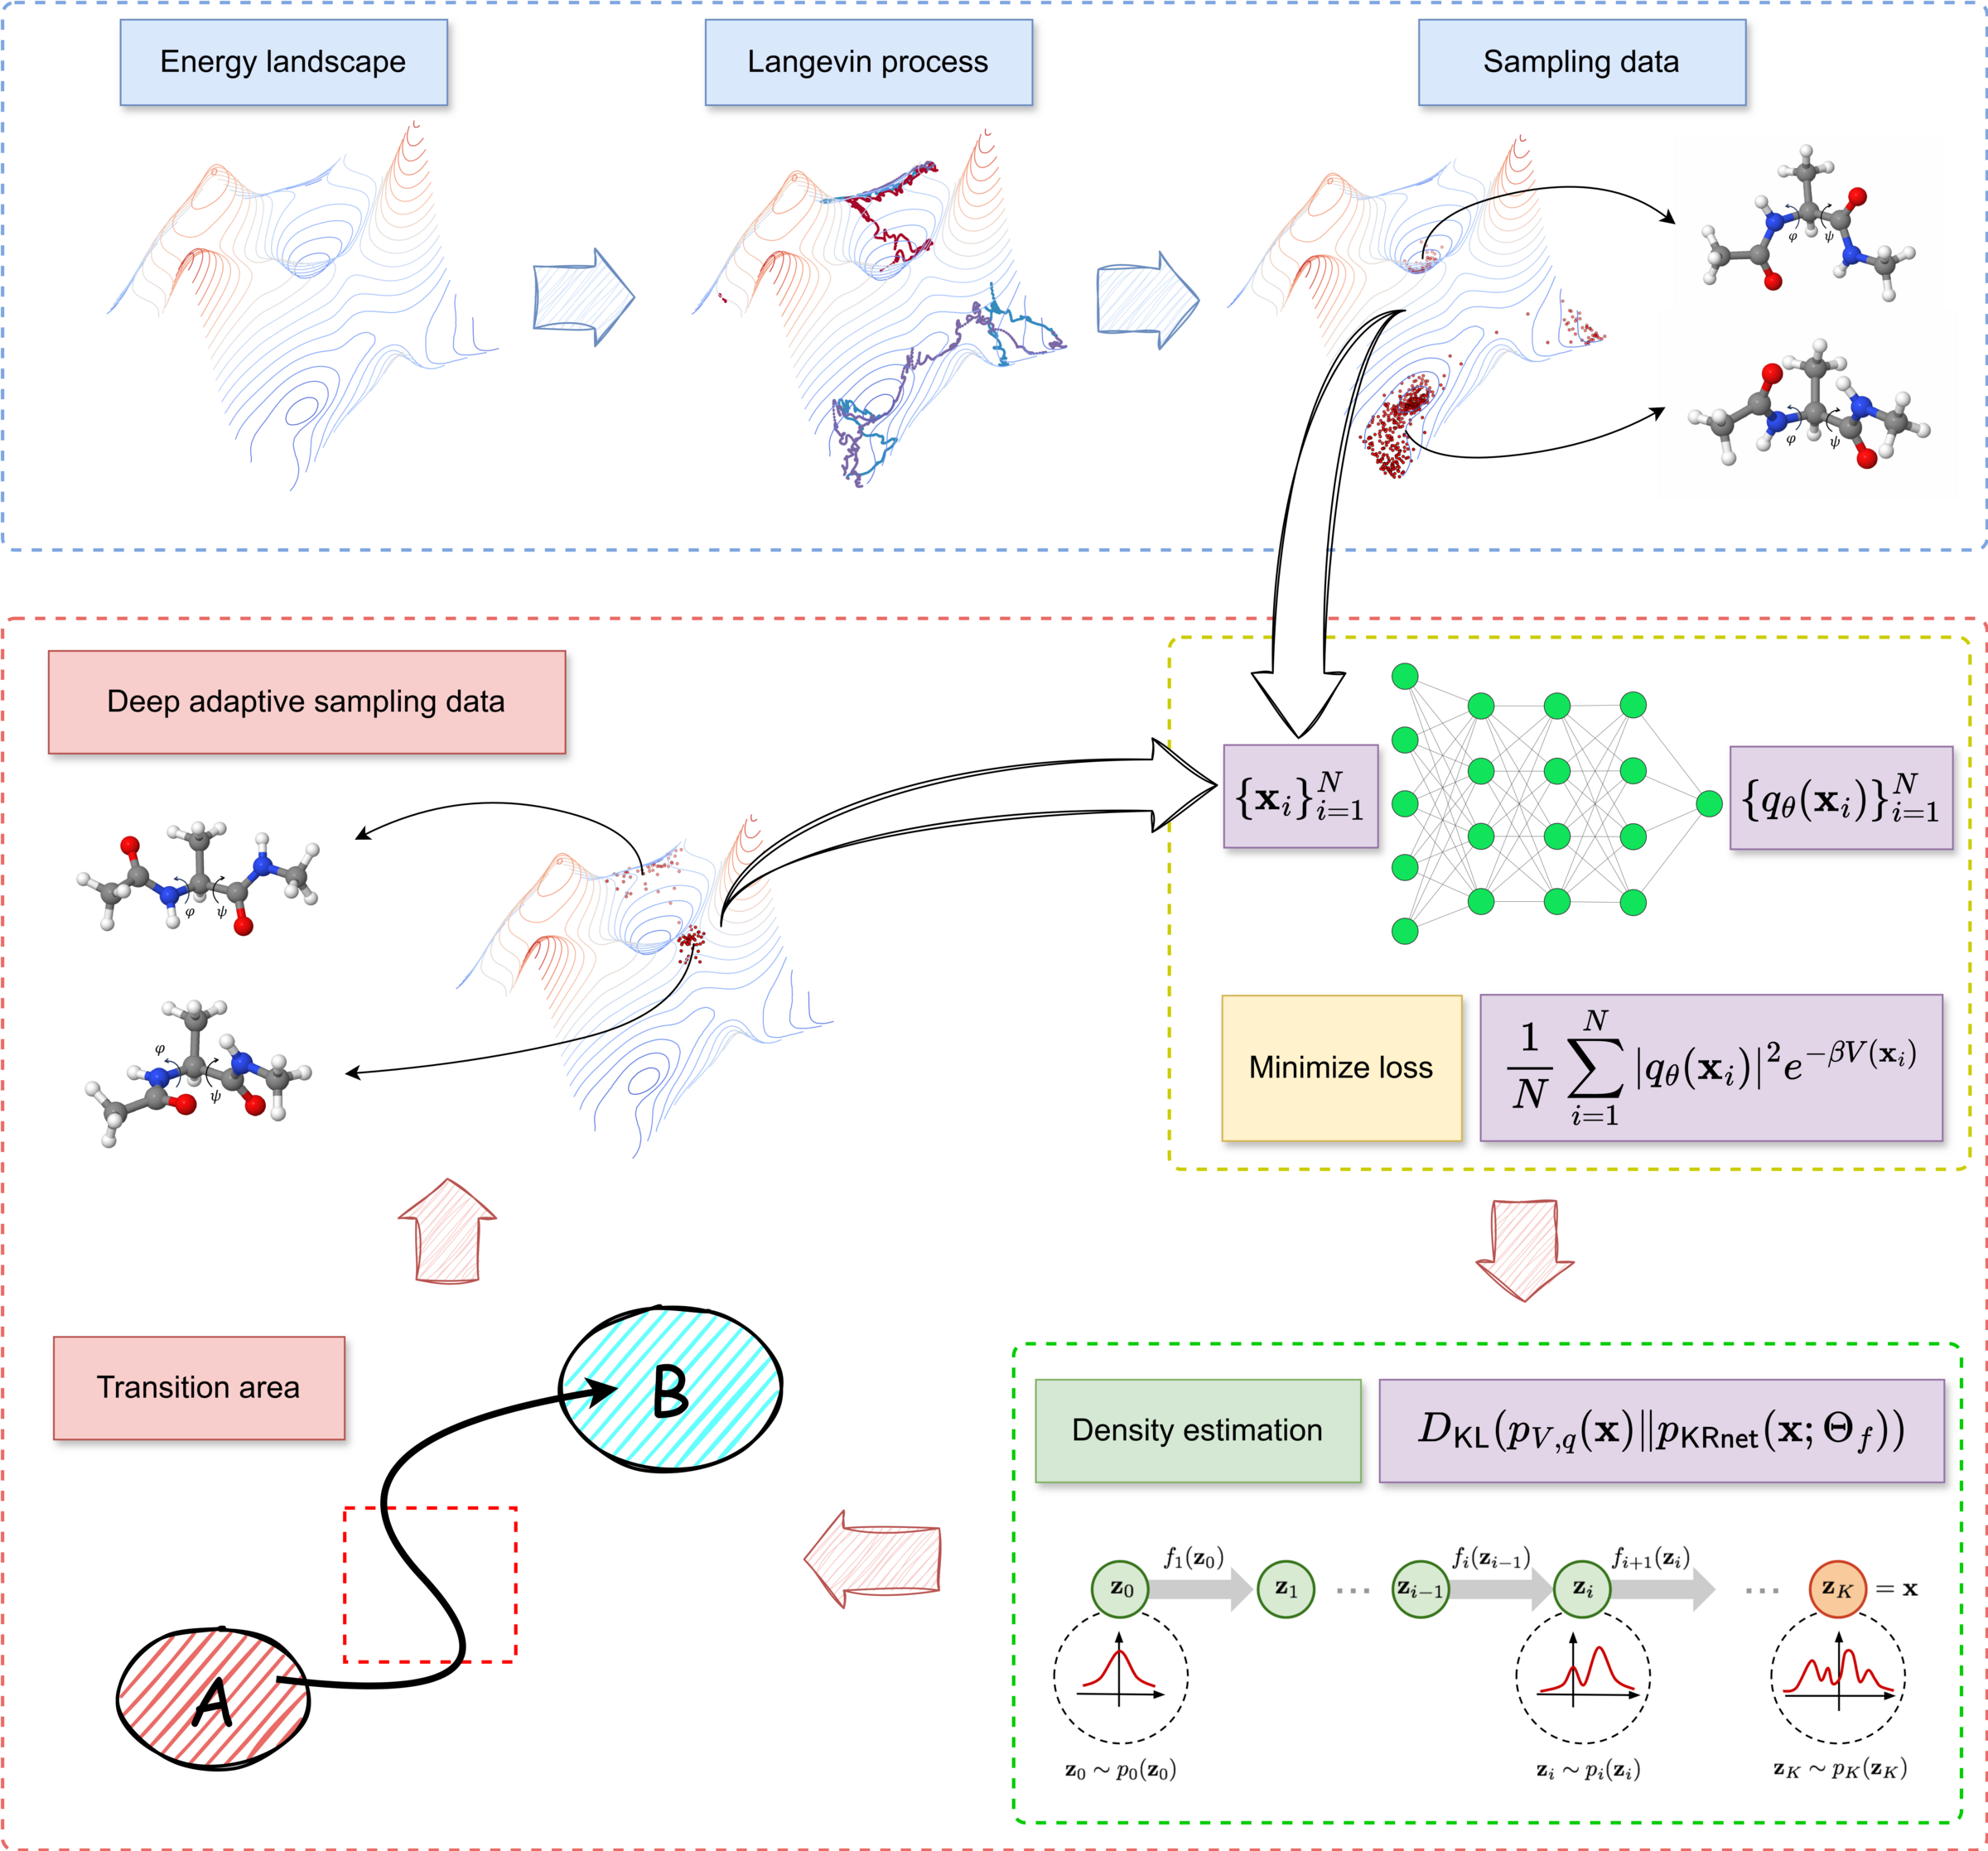
\includegraphics[width=0.72\textwidth]{img/dastr-workflow.png}
  \caption{The DASTR feedback loop: ordinary dynamics undersample rare
  transitions, so a generative density model produces additional transition
  points for the next committor update.  Reproduced from Figure~1 of
  \href{https://arxiv.org/abs/2501.15522}{Wang et al.}}
  \label{fig:dastr-workflow}
\end{figure}

The representation used by the sampler also matters.  In
Figure~\ref{fig:dastr-representation}, direct sampling in the full molecular
coordinate space breaks correlations between atoms and produces invalid
configurations.  Sampling in a lower-dimensional space of latent collective
variables preserves the relevant molecular geometry.  The same lesson applies
to certificate training: adaptive samples must both target difficult regions
and remain valid states of the original problem.

\begin{figure}[htbp]
  \centering
  \begin{minipage}{0.47\textwidth}
    \centering
    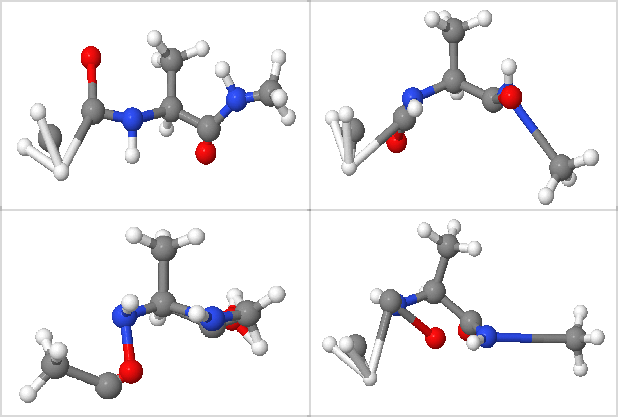
\includegraphics[width=\linewidth]{img/dastr-direct-coordinates.png}
    \small (a) Direct molecular coordinates
  \end{minipage}
  \hfill
  \begin{minipage}{0.47\textwidth}
    \centering
    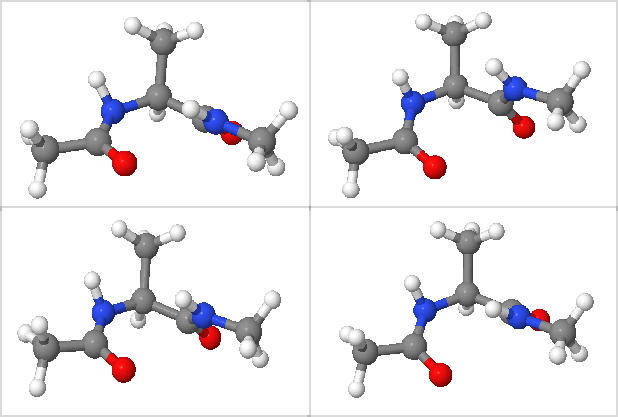
\includegraphics[width=\linewidth]{img/dastr-latent-coordinates.png}
    \small (b) Latent collective variables
  \end{minipage}
  \caption{Samples generated in two DASTR representations.  Direct-coordinate
  sampling gives mostly invalid structures; latent-coordinate sampling gives
  physically consistent structures.  Reproduced from Figure~2 of
  \href{https://arxiv.org/abs/2501.15522}{Wang et al.}}
  \label{fig:dastr-representation}
\end{figure}

The same principle can support certificate training.  A learned committor can
identify transition regions, and training can place more points there together
with known verifier counterexamples.  However, the committor itself is not a
certificate: it satisfies $\mathcal Lq=0$, while the certificate requires the
strict inequality $\mathcal LV\leq-\epsilon$.  It should therefore be used only
as a teacher or sampling guide.  The final guarantee must still come from a
construction-safe model and a formal verifier.

\clearpage

\section{Summary and takeaways}

\begin{enumerate}
  \item The Residual Deep ICNN architecture is still promising, since:
  \begin{enumerate}
    \item We don't have to check the local-time sign condition on every facet 
    \item I managed to formally verify it by optimizing with \textbf{Linear Programming} 
    (infeasible in the long run.)
    \item I managed to optimize it with \textbf{Adam}, but required 100x parameters and 
    couldn't verify it formally (it looks )  (feasible in the long run.)
  \end{enumerate}
  \item I should have listened to Greg and used IBP instead of cell discovery for verification.
  Cell discovery would take $2 \cdot 10^{15}$ years.
  \item IBP through ReLUs is still potentially faster than through smooth activations  
  \item Committor functions are not directly useful here, but they can help with training 
  hard certificates by guiding sampling
\end{enumerate}

\end{document}
